\chapter{Framework}
\label{chap:framework}

This chapter cover the design framework developed from the Theoretical background and best practice evaluation. In the following sections we propose how each component of the framework contribute to a good onboarding experience. The framework is conceptualized around the organizational onboarding definition of Bradt. et al \cite{Bradt2009}, which constitute that onboarding is a process of \textit{acquiring}, \textit{accommodating}, \textit{assimilating} and \textit{accelerating} new members (see Figure \ref{fig:process}). Psychological, behavioral and UX research is cited to be able to facilitate a thorough understanding of how humans reason, learn and accomplish with mobile interfaces. With this framework, designers will be better equipped when designing onboarding experiences for mobile users.

\begin{figure}[h]
  \centering
    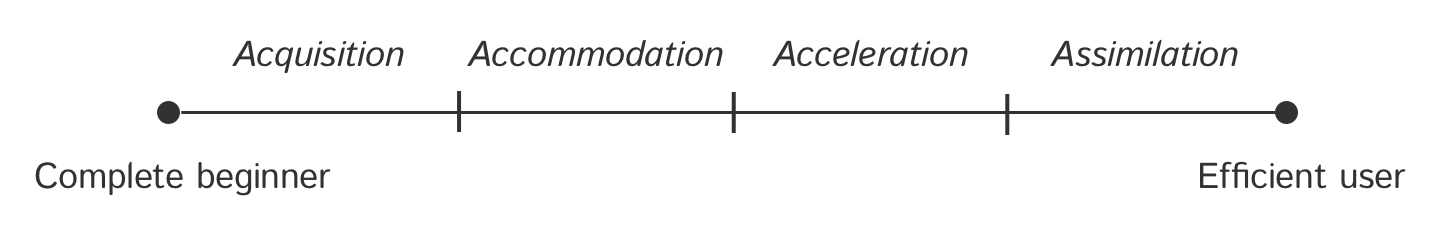
\includegraphics[width=0.8\textwidth]{presentation/Timeline}
  \caption{Onboarding process.}
  \label{fig:process}
\end{figure}

\section{Acquisition}
There's a lot that determine the willingness for an individual to use and adopt some piece of technology. For this section we will present some aspects that affect this willingness.

\subsection{Adoption process}

The adoption process of a user follows five steps; \begin{enumerate*}[label=(\(\arabic*\))]
  \item knowledge,
  \item persuasion,
  \item decision,
  \item implementation and
  \item confirmation,
\end{enumerate*} all of which are explained further in the following subsections below.

\subsubsection{Knowledge}

Knowledge is when an individual first gathers knowledge about the mobile app. They may hear about the app from a friend, or through an advert or by actively looking for a product that satisfy one of the needs of the user. Research by Google and Ipsos has found that apps are often discovered outside the app store; 52\% hear about apps through their family, friends and colleagues, 40\% browse the app store, 27\% use some sort of search engine, 24\% from company website and 22\% through TV \cite{Tiongson2015}.

After learning about the existence of the app the person may ask questions such as "What is the app?", "How does the app work?" and "Why does it work?". While answering these questions they may acquire \textit{how-to knowledge} and \textit{persuasion knowledge}. How-to knowledge is knowledge about how to use the app and may be acquired through word-of-mouth, reading about the application online or reading its description on the application store of the corresponding mobile platform. Persuasion knowledge is about understanding \textit{how the app works}. This type of knowledge may be harder to acquire, but it is usually not required by the user to use the app.

\subsubsection{Persuasion}

Persuasion is when the person form a favorable or unfavorable attitude toward the usage of the  mobile app. When this happens, the person are thinking about how they can apply the app to their current situation, and if it meets their needs. At this stage, the person may ask questions such as "What are the app's consequences?" and "What will its advantages and disadvantages be when I apply it to my situation?". Here, peer opinion is important to person. If a friend or relative has had positive experiences with the mobile app they are more likely to form a favorable opinion about it.

Forming an intention to use the mobile app is based on two major beliefs; \textit{perceived ease of use} and \textit{perceived usefulness}. Perceived ease of use is how much the person believes that using the mobile app will be free of effort and easy to use. Perceived usefulness is how much a person believes that using the app will improve their life. These two beliefs affect each other; when an app is easy to use it can be more useful.

What are some determinants of perceived ease of use and perceived usefulness? Research has identified some:
\begin{description}
  \item[Control] -
  \item[Intrinsic motivation] - Explain, point to section
  \item[Emotion] - Explain
\end{description}

It is also worth to point out that perceived ease of use and perceived usefulness are not only determined by the mobile app itself, but also by the persons prior experience with either similar apps and their general experience with using mobile apps. If they have had negative experiences before with a similar app they are more likely to form an unfavorable opinion about the apps perceived ease of use and perceived usefulness, affecting the behavioral intention to use it.

\subsubsection{Decision}
The decision process leads the person to the decision whether or not to become a user of the app. This decision is usually made after the person has tried using the app if there's either a trial or free version. If the app cost money to download it must be adopted or rejected in its entirety, and is harder to adopt.

\ignore{
occur when the individual engage in activities which will either lead the person to either adopt or reject the innovation. This means for most individuals to try out the new innovation at least partially. This time period as they apply the innovation is often part of the decision to adopt, and its important during this time to decrease the uncertainty of the value to the possible adopter. An accessible trial period of the innovation, e.g. a free sample or free time period, are generally adopted more rapidly compared to an innovation that must be adopted or rejected in its entirety. It is important to remember though that
}

\subsubsection{Implementation}
Even though a person has decided to download and use an app, actually putting it to use is a whole other thing. For a target behavior to occur (in our case for the person to use the app regularly) the person needs the \textit{motivation} and \textit{ability} to do so. Motivation can be categorized into \textit{intrinsic} and \textit{extrinsic} motivation. Intrinsically motivated people are motivated to do something due to the task being interesting or fun, like playing a video game, while extrinsically motivated people are motivated to do something to achieve a specific external goal, like taking a shower. Extrinsic motivation can be powerful, but when the external reward is removed so does the motivation. It has been found that intrinsically motivated people perform have a higher willingness to spend more time on a task. These categories are not mutually exclusive; a person may be both intrinsically and extrinsically motivated.

To improve the users intrinsic motivation, the user interface designer can relate the content and objectives of the application to the needs and interests of the learner \ignore{\cite{Keller1983}}. This can be done by using familiar metaphors and analogies \ignore{\cite{Curtis1984}}. Instructions provided to the user that use a personal style (e.g personal pronouns, names of specific people) rather than formal style may stimulate the user to learn. Also, providing immediate, positive and informative feedback in a context may improve intrinsic motivation, but not necessarily increase or decrease performance \ignore{\cite{(Bates, 1979; Condry, 1977; Deci, 1975, 1971; Keller, 1983)}}. Humor, on the the other hand, has been found to not improve motivation since it can distract the user and interfere with comprehension \ignore{\cite{Markiewicz, 1974; Sternthal & Craig, 1973}}.

Increasing the motivation of the user is not always the solution to make them perform a target behavior or use your mobile app. Sometimes increasing the users ability to perform the target behavior (making it easier to perform), or increasing the perceived ease of use, is the solution.

While some amount of motivation and ability is required for the user to perform some task, a trigger is required to remind the user to perform the task. Fogg has identified three categories of triggers that help the user

\begin{description}
  \item[Spark as Trigger] High ability/Low motivation, the \textit{spark} should try and motivate the user to perform the behavior.
  \item[Facilitator as Trigger] Low ability/High motivation, the \textit{facilitator} should try and make the target behavior easier to perform.
  \item[Signal as Trigger]  High ability/High motivation, the \textit{signal} should only remind the person to perform the target behavior.
\end{description}

Here are some examples of implemented triggers in mobile applications.

\begin{figure}
\centering
\captionsetup{format=multiline,font=footnotesize}
\begin{minipage}{.33333\textwidth}
  \centering
  \includegraphics[noincl, width=\linewidth,height=8cm]{triggers/spark.png}%
  \caption{\\Spark as Trigger}
  \label{fig:spark}
\end{minipage}%
\begin{minipage}{.33333\textwidth}
  \centering
  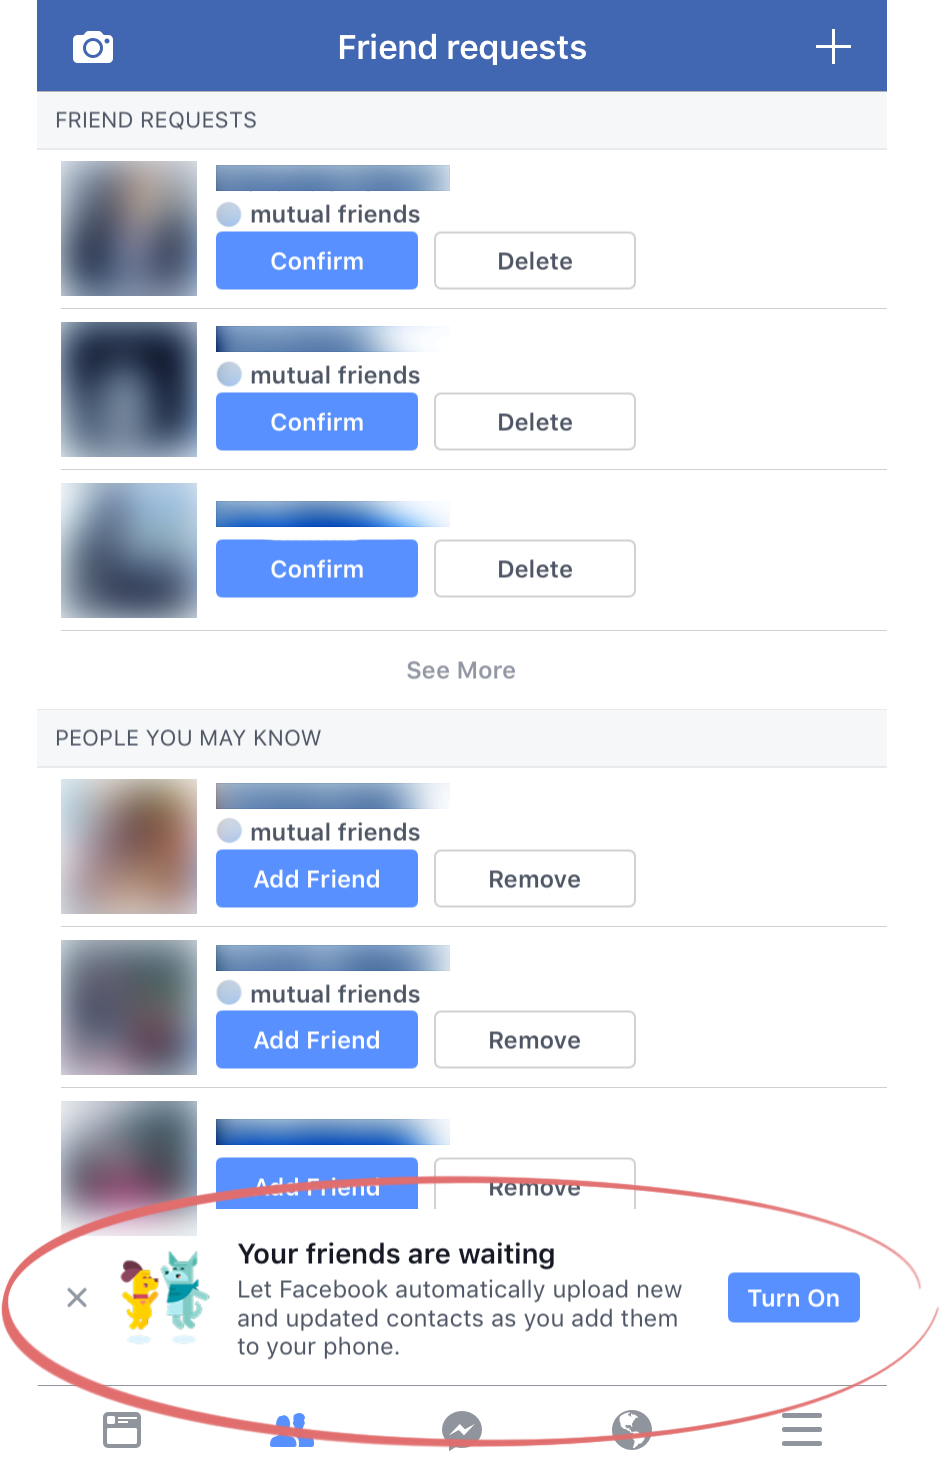
\includegraphics[width=\linewidth]{triggers/facilitator.png}%
  \captionof{figure}{\\Facilitator as trigger}
  \label{fig:facilitator}
\end{minipage}%
\begin{minipage}{.33333\textwidth}
  \centering
  \includegraphics[noincl, width=\linewidth, height=8cm]{triggers/signal.png}%
  \captionof{figure}{\\Signal as trigger}
  \label{fig:signal}
\end{minipage}
\end{figure}

To be able to help the user perform a task we need to think about what influences the difficulty of a task.

\begin{description}
  \item[Time] If the user does not have the time to perform a task, the task will not be easy to perform. (e.g. )
  \item[Money] If the user does not have the money or resources to perform a task it will not be easy to perform. (e.g. )
  \item[Physical Effort] Behaviors that require physical effort may not be easy to perform. If the physical effort is small, the easier it is for the people to perform the behavior. It is important at this stage to consider the different physical disabilities of your target market.
  \item[Brain cycles] A task that is demanding the user to think hard about it might lead the person to think that it is difficult to perform. In some cases the task at hand might not itself be hard to think about, but the persons mind might be consumed with other issues at the same time.
  \item[Social deviance] If the task required the person to go against the norm, breaking the rules of society, the behavior is not simple to perform.
  \item[Non-routine] People tend to think that activities they perform on a routine to be easy, like brushing your teeth, while new activities might be hard to perform. While seeking simplicity, the person might resort to perform a task that they are more familiar with instead.
\end{description}

These aspect might influence us differently. For example, a person that is on a rush to catch the bus will believe that performing any other task will be difficult. The one aspect that we have the most limited resources of when a behavior is triggered will determine how difficult the task is.

Even though with the mobility of smartphones, its wide range of possible uses and the big opportunity of using contextual triggers we must be vary of the triggers we use. Sparks may annoy us because they will try and motivate for a behavior that we do not want to perform. Users will be most tolerant of triggers when they act as signals or facilitators.

\subsubsection{Confirmation}

The final stage of adoption is the \textit{confirmation} stage. At this stage the individual will seek confirmation that their choice to use an app is correct, but if the individual find conflicting messages about the app they will experience \textit{dissonance}. The feeling of dissonance is unpleasant to the user, and will try to avoid by either changing their beliefs, attitude or knowledge. The person may avoid dissonance by only seeking information that support their decision to adopt or avoid information that is not consistent with the persons beliefs. Avoiding conflicting messages can still reach the individual, even if they avoid it, and they may doubt their decision to use the app. Examples of conflicting messages might a opinion from a friend or bad ratings of the app.

\subsection{User research}
To successfully satisfy the need of your user with your app you need to identify the need they are trying to satisfy. This implicitly means that you have to identify you user-base and in what context they will be using your mobile app. In the product development cycle, this is usually done through \textit{user research}.

User research focuses on understanding user behaviors, needs and motivations through different observation techniques\footnote{\url{https://www.usability.gov/what-and-why/user-research.html}}. While there are plenty of different methods for learning about your users, we will endorse creating \textit{personas} to represent your target market.

\section{Accommodation}

\section{Acceleration}

\section{Assimilation}
